\newpage
{\bfseries ҒТАМР 65.65.29}
\hfill {\bfseries \href{https://doi.org/10.58805/kazutb.v.2.23-472}{https://doi.org/10.58805/kazutb.v.2.23-472}}

\sectionwithauthors{А.Е. Отуншиева, С.А. Болегенова, С.А. Ламоткин, С.С. Ветохин, А.А. Ешанкуло}{ҚАЗАҚСТАНДЫҚ МАҚТА МАЙЫ ЖӘНЕ РЕСЕЙЛІК АРЫШ МАЙЫНЫҢ НЕГІЗІНДЕ
ТЕҢЕСТІРІЛГЕН МАЙ ҚЫШҚЫЛДЫ ҚҰРАМЫ БАР ӨСІМДІК МАЙЛАРЫ ҚОСПАЛАРЫНЫҢ ЖАҢА
ТҮРЛЕРІН ӘЗІРЛЕУ}

\begin{center}
{\bfseries \textsuperscript{1}А.Е. Отуншиева, \textsuperscript{1}С.А. Болегенова, \textsuperscript{2}С.А. Ламоткин, \textsuperscript{2}С.С. Ветохин, \textsuperscript{3}А.А. Ешанкуло}

\textsuperscript{1}Әл-Фараби атындағы Қазақ Ұлттық университеті КеАҚ,
Алматы, Қазақстан,

\textsuperscript{2}Беларусь мемлекеттік технологиялық университеті,
Минск, Беларуссия,

\textsuperscript{3}М.Әуезов атындағы Оңтүстік Қазақстан Зерттеу
университеті, Шымкент, Қазақстан,

Корреспондент-автор: 03.08.1990.43@mail.ru
\end{center}

Мақалада қазіргі тамақ өнеркәсібінде дұрыс тамақтану үшін жаңа қоспалар
түрі ұсынылған. Дұрыс тамақтану қағидалары мен ережелерін ұстануда адам
ағзасы үшін биологиялық құндылық тұрғысынан функционалдық бағдарланған
тамақ өнімдерінің, оның ішінде май өнімдерінің жаңа түрлері әзірленуде.
Құрамында ω-6 және ω-3 май қышқылдары әртүрлі (мақта, жүгері, рапс және
зығыр) өсімдік майларының құрамы қарастырылады. Жеке майлардың
полиқанықпаған май қышқылдарының сапалық және сандық құрамы газ
хроматографиясының көмегімен зерттелді. Жеке майлардағы май
қышқылдарының арақатынасы оңтайлы емес екені анықталды. Мақта және арыш
майларындағы жеке май қышқылдарының сандық құрамы негізінде ω-3 және ω-6
май қышқылдарының арақатынасы 10:1 және 5:1 болатын қоспаларды алу үшін
осы майлардың қоспаларының оңтайлы құрамы есептелді. Алынған өсімдік
майларының қоспаларының үлгілері олардың органолептикалық және
физико-химиялық көрсеткіштерін анықтау үшін зерттеулерден өтті . Сонымен
қатар, алынған қоспалардың өлшенген сапа көрсеткіштері (қышқыл және
асқын тотық мәндері) стандартталған мәндерден аспайды. Өсімдік
майларының әзірленген мақта-арыш қоспаларында дұрыс тамақтану үшін
ұсынылған деңгейлерге сәйкес келетін ω-6 және ω-3 полиқанықпаған май
қышқылдары бар және өсімдік майлары негізінде тағамдық қоспалар жасау
үшін пайдаланылуы мүмкін.

{\bfseries Түйін сөздер:} өсімдік майлары, мақта майы, арыш майы,
биологиялық белсенді қоспалар, газ-сұйықтық хроматографиясы, линол және
линолен қышқылдары, полиқанықпаған май қышқылдары.

\begin{center}
{\large\bfseries DEVELOPMENT OF NEW TYPES OF BLENDS OF VEGETABLE OILS WITH
BALANCED FATTY ACID COMPOSITION ON THE BASIS OF KAZAKH COTTON OIL AND
RUSSIAN LIVERWORT OIL}

{\bfseries \textsuperscript{1}A.E. Otunshiyeva, \textsuperscript{1}S.А.
Bolegenova, \textsuperscript{2}S.A. Lamotkin, \textsuperscript{2}S.S.
Vetokhin,}

{\bfseries \textsuperscript{3}A.A. Yeshankulov}

\textsuperscript{1}Al-Farabi Kazakh National University, Almaty,
Kazakhstan,

\textsuperscript{2}Belarusian State Technological University, Minsk,
Belarus,

\textsuperscript{3}M. Auezov South Kazakhstan Research University,
Shymkent, Kazakhstan,

e-mail: 03.08.1990.43@mail.ru
\end{center}

At present, new types of food products are being developed, including
fatty foods, functionally oriented in terms of biological value for the
human body, adhering to the principles and rules of healthy nutrition.
The compositions of vegetable oils containing various ω-6 and ω-3 fatty
acids (cotton, corn, rapeseed and linseed) are considered. The
qualitative and quantitative composition of polyunsaturated fatty acids
of individual fats was investigated by gas chromatography. It was found
that the ratio of fatty acids in the individual oils was not optimal.
Based on the quantitative composition of individual fatty acids in
cottonseed and lynx oils, the optimal composition of blends of these
oils was calculated to obtain blends in which the ratio of ω-3 and ω-6
fatty acids is 10:1 and 5:1. Samples of the obtained vegetable oil
blends were tested to determine their organoleptic and physicochemical
parameters. At the same time, the measured quality indicators of the
obtained blends (acidity and peroxide values) do not exceed the
standardised values. The developed cotton blends of vegetable oils
contain polyunsaturated fatty acids ω-6 and ω-3, corresponding to the
recommended levels for a healthy diet, and can be used to create food
additives based on vegetable oils.

{\bfseries Keywords:} vegetable oils, cottonseed oil, lynghorn oil,
biologically active additives, gas-liquid chromatography, linoleic and
linolenic acids, polyunsaturated fatty acids.

\begin{center}
{\large\bfseries РАЗРАБОТКА НОВЫХ ВИДОВ КУПАЖЕЙ РАСТИТЕЛЬНЫХ МАСЕЛ СО СБАЛАНСИРОВАННЫМ ЖИРНОКИСЛОТНЫМ СОСТАВОМ НА ОСНОВЕ КАЗАХСТАНСКОГО ХЛОПКОВОГО МАСЛА И РОССИЙСКОГО РЫЖИКОВОГО МАСЛА}

{\bfseries \textsuperscript{1}А.Е. Отуншиева, \textsuperscript{1}С.А.
Болегенова, \textsuperscript{2}С.А. Ламоткин, \textsuperscript{2}С.С.
Ветохин,}

{\bfseries \textsuperscript{3}А.А. Ешанкулов}

\textsuperscript{1}Казахский национальный университет имени аль-Фараби,
Алматы, Казахстан

\textsuperscript{2}Белорусский государственный технологический
университет, Минск, Беларусь,

\textsuperscript{3}Южно-Казахстанский исследовательский университет
им.М.Ауэзова, Шымкент, Казахстан,

e-mail: 03.08.1990.43@mail.ru
\end{center}

В настоящее время разрабатываются новые виды продуктов питания, в том
числе жировые, функционально ориентированные с точки зрения
биологической ценности для организма человека, придерживающиеся
принципов и правил здорового питания. Рассмотрен состав растительных
масел с различным содержанием ω-6 и ω-3 жирных кислот (хлопковое,
кукурузное, рапсовое и льняное). Изучен качественный и количественный
состав полиненасыщенных жирных кислот индивидуальных масел методом
газовой хроматографии. Установлено, что соотношение жирных кислот, в
индивидуальных маслах не является оптимальным. На основе количественного
содержания индивидуальных жирных кислот в хлопковом и рыжиковом маслах,
проведен расчет оптимального состава смесей этих масел для получения
купажей с соотношением ω-3 и ω-6 жирных кислот 10:1 и 5:1. Измеренные
показатели качества (кислотное и перекисное число) полученных купажей не
превышают нормируемых значений. Разработанные хлопково-рыжиковые купажи
растительных масел содержат ω-6 и ω-3 полиненасыщенные жирные кислоты на
уровне, соответствующем рекомендуемому для питания, и могут быть
использованы для создания биологически активных добавок на основе
растительных масел.

{\bfseries Ключевые слова:} растительные масла, хлопковое масло, рыжиковое
масло, биологические активные добавки, газожидкостная хроматография,
линолевая и линоленовая кислоты, полиненасыщенные жирные кислоты.

\begin{multicols}{2}
{\bfseries Кіріспе.} Майлар мен тоң майлардың тамақ өндірісінде кеңінен
қолданылуы олардың ерекше қасиеттеріне байланысты. Бұл ингредиенттер
өнімге белгілі бір консистенция мен жағымды құрылымды береді және тез
қанықтыруға ықпал етеді. Сонымен қатар, майлар мен тоң майлар әдетте хош
иістендіргіш заттардың тасымалдаушысы ретінде қызмет етеді.

Майлар мен тоң майлар ақуыздар мен көмірсулармен қатар адам диетасының
маңызды құрамдас бөлігі болып табылатын липидтердің негізгі кластары
болып табылады. Олардың тағамдық құндылығы май қышқылдарының құрамымен,
сондай-ақ, триацилглицерин молекуласындағы май қышқылдарының таралуымен
анықталады. Липидтердің адам ағзасына түсуінің негізгі көзі өсімдік
майлары және олардан тұратын тағам өнімдері болып табылады {[}1{]}.

Май-тоңмай өнеркәсібі май өндіру және май өңдеу кәсіпорындарымен
ұсынылған. Ол Қазақстан Республикасы халқының азық-түлікке сұранысын
қанағаттандыруда маңызды рөл атқарады, сонымен қатар, бірқатар өнеркәсіп
салалары (балық аулау, кондитерлік, нан пісіру, бояу-лак, мұнай-химия)
үшін өндіріске қажетті шикізатпен қамтамасыз етеді. Салалық ұйымдар
өсімдік майы, майонез және маргарин өнімдерін, шаруашылық және иіс сабын
өндіруге маманданған. Өсімдік майы стратегиялық өнім болып табылады,
оның өндірісі азық-түлік секторында импортты азайтуға және экспортты
арттыруға алғышарттар жасайды.

Қазіргі уақытта май-тоңмай өнеркәсібінің жұмысы республиканың өсімдік
майымен және дайын өніммен өзін барынша қамтамасыз етуге бағытталған.
Бірқатар майлы дақылдарды өсіруге қолайлы климаттық жағдайлардың болмауы
күнбағыс, арыш және өсімдік майының басқа да кейбір түрлерін
импорттаудан толық бас тартуға мүмкіндік бермейді.

Халықтың жекелеген топтарының, соның ішінде балалардың нақты тамақтануын
кешенді медициналық-гигиеналық зерттеулер тамақтағы негізгі қоректік
заттар мен энергияны қабылдаудың теңгерімсіздігін, атап айтқанда,
маңызды биологиялық функциялар атқаратын полиқанықпаған май қышқылдарын
(ПҚМҚ) тұтынудың төмен деңгейін көрсетті {[}2{]}.

Маңызды емес қоректік факторлардың бірі болып табылатын полиқанықпаған
май қышқылдары (ПҚМҚ) біздің елімізде де, шетелде де зерттеушілердің
назарын аударды. Соңғы онжылдықтарда бұл қосылыстардың қалыпты дамудағы
және организмдегі физиологиялық және патологиялық процестер арасындағы
тепе-теңдікті сақтаудағы маңызды рөлін көрсететін дәлелдер жинақталды.

Май қышқылдары екі үлкен топқа бөлінеді: қаныққан, олар бір
(моноқанықпаған) немесе қос және бірнеше байланысы бар (поли
қанықпаған). Қанықпаған май қышқылдары гректің ω әрпімен белгіленген
қанықпаған май қышқылдарының метил тобының соңғы көміртегі атомына
қатысты қос байланыстың орнына байланысты қанықпаған май қышқылдарының
бірнеше негізгі тұқымдастарын ажыратады: омега-9, омега-6 және омега-3.
Қанықпаған май қышқылдарының ішінде омега-3 және омега-6 май қышқылдары
ω-6 позициясында қос байланыстың түзілуін катализдейтін ферменттік
жүйенің болмауына байланысты организмде синтезделе алмайды. Осылайша,
линол қышқылы мен b-линолен қышқылы (ALA) организмде синтезделе алмайды.
Олар алмастырылмайтын май қышқылдары болып табылады және оларды тамақпен
қамтамасыз ету керек {[}3{]}.

ПҚМҚ теңгерімді тұтыну денсаулықты сақтауға және жақсартуға, сондай-ақ,
халық арасында созылмалы инфекциялық емес аурулардың өсуіне жол бермеуге
көмектеседі {[}4, 5{]}. Бұл принципті жүзеге асыруға үлкен кедергі болып
полиқанықпаған май қышқылдарының физиологиялық белсенді заттар болғанына
қарамастан оларды еркін тұтыну болып табылады. Бұл мәселені шешудің бір
жолы -- биологиялық белсенді қоспаларды (ББҚ) әзірлеу және ω-3 және ω-6
полиқанықпаған май қышқылдарын қосу арқылы тамақ өнімдерін байыту болып
табылады.

Белгілі болғандай, ω-6 полиқанықпаған май қышқылдарына линол қышқылы
(С18: 2, ω-6) жатады, ол организмде арахидон қышқылына (С20:4, ω-6)
айналады. Арахидон қышқылы (АҚ) линол қышқылының жетіспеушілігі болған
кезде ғана ағзаға қажет. Омега-6 және омега-3 қатарындағы полиқанықпаған
май қышқылдары негізгі тағамдық көзі болып табылатын өсімдік майлары
болып табылады 1-кестеде келтірілген {[}3,4{]}.
\end{multicols}

\begin{table}[H]
\caption*{1-кесте - Өсімдік майларындағы омега-3 және омега-6 май қышқылдарының мөлшері мен арақатынасы}
\centering
\resizebox{\textwidth}{!}{%
\begin{tabular}{|l|l|l|l|}
\hline
Май атауы & Өнімдегі омега-3, г/100 г & Өнімдегі омега-6, г/100 г & Омега-3:омега-6 қатынасы \\ \hline
Зығыр майы & 53 & 17 & 1:0,3 \\ \hline
Арыш майы & 35–38 & 28–38 & 1:0,8–1:1 \\ \hline
Сора майы & 26 & 54 & 1:2 \\ \hline
Балқарағай майы & 16 & 37 & 1:2,3 \\ \hline
Грек жаңғағының майы & 10,5 & 53 & 1:5 \\ \hline
Рапс майы & 9 & 14,5 & 1:6 \\ \hline
Соя майы & 7 & 50 & 1:7 \\ \hline
Қыша майы & 5,9 & 15 & 1:2,5 \\ \hline
Амарант майы & 1,8 & 50 & 1:28 \\ \hline
Жүгері майы & 1,16 & 53,5 & 1:46 \\ \hline
Авокадо майы & 0,96 & 12,5 & 1:13 \\ \hline
Зәйтүн майы & 0,76 & 9,7 & 1:13 \\ \hline
Кунжут майы & 0,3 & 41,3 & 3:17 \\ \hline
Пальма майы & 0,2 & 9,1 & 1:46 \\ \hline
Күнбағыс майы & 0,2 & 40 & 4:20 \\ \hline
Мақта майы & 0,2 & 51,5 & 5:17 \\ \hline
\end{tabular}%
}
\end{table}

\begin{multicols}{2}
Жалпы, дені сау адам үшін дұрыс тамақтануды ұстану жеткілікті. Майлар
мен тоңмайларды өнеркәсіптік өңдеу біздің диетамыздағы алмастырылмайтын
май қышқылдарының құрамын айтарлықтай төмендетті. Диетада маңызды май
қышқылдары дененің жалпы калория қажеттілігінің кем дегенде 1-2\%
(калория мөлшері бойынша) құрауы керек. Азық-түліктегі ω-3: ω-6 май
қышқылдарының оңтайлы қатынасы 1:(3...5). Адамның линол қышқылына ең
төменгі тәуліктік қажеттілігі 2-6 г құрайды, бірақ бұл қажеттілік денеге
түсетін қаныққан майлардың үлесіне пропорционалды түрде артады {[}6,
7{]}.

Қазіргі уақытта «салауатты» азық-түлік өнімдері барлық белгілі
азық-түлік өнімдерінің 3\%-дан аспайды. Алдағы бір-екі онжылдықта бұл
өнімдерге еуропалық нарықтың әлеуеті бойынша сатылған барлық азық-түлік
өнімдерінің 30\%-дан асады деп болжануда. Маркетингтік агенттіктің
зерттеулеріне сәйкес, «салауатты» азық-түлік секторындағы ең қарқынды
дамып келе жатқан өнім топтары сүт және май-тоңмай өнімдері болып
табылады, сондықтан пайдалы май-тоңмай өнімдерінің ассортиментін
кеңейтудің болашағы зор.

Майлардың құрамын жетілдіру қажеттілігі белгілі тағамдық майлардың
ешқайсысының идеалды май туралы заманауи идеяларға сәйкес
келмейтіндігінен туындады:

-- табиғи майлар мен майлардағы май қышқылдарының теңдестірілген құрамы
жоқ, сондықтан адам рационы үшін ω-6 және ω-3 тұқымдасының қаныққан,
моно және полиқанықпаған май қышқылдарының оңтайлы арақатынасы жоқ;

-- тазартылған майлар, олардың даусыз дәмдік артықшылықтары мен жоғары
тұтынушылық сипаттамаларына қарамастан, фосфолипидтерге, Е
витаминдеріне, фитостеролдарға, каротиноидтарға және басқа да
физиологиялық құнды қосылыстарға нашар;

- тазартылмаған майлардың құрамында көрсетілген микроэлементтер бар,
сонымен қатар, майлардың тағамдық құндылығын төмендететін және оларды
тағамдық технологияда қолдануды қиындататын қажетсіз ілеспе заттар бар
{[}8{]}.

Май қышқылдарының құрамын өзгерту қажеттілігінің тағы бір себебі --
құрамында май қышқылдарының транс-изомерлері жоқ май өнімдерінің дамуы,
оларды тұтыну адам денсаулығына елеулі қауіп факторы болып табылады.

Өсімдік майларын араластыру -- табиғи өсімдік майларынан екі немесе көп
компонентті жүйелер құру арқылы әртүрлі типтегі май қышқылдарының
берілген қатынасына жетудің тиімді технологиялық әдісі. Қоспада
тазартылған дезодорацияланған майлар (күнбағыс, мақта, соя, рапс,
жүгері, арыш тұқымы) және тазартылмаған (күнбағыс, мақта, зығыр, арыш
майы, бидайық майы) қолданылады {[}9{]}. Аралас майдың сапасын
қамтамасыз ететін факторлардың бірі оның дәмдік және хош иісті
қасиеттері болып табылады. Мұндай қоспалары құрамының құрамдас
бөліктерін және оларды дайындау технологиясын есептеу ω-6 және ω-3
тұқымдасының полиқанықпаған май қышқылдары қажетті теңдестірілген құрамы
бар май негізін алуға мүмкіндік береді {[}9{]}.

Майлы өнімдерді функционалдық өнімдер ретінде пайдалануды кеңейту тамақ
өнеркәсібін дамытудың перспективті бағыттарының бірі болып табылады, бұл
жаңа функционалдық өнімдерді жасау үшін инновациялық шешімдерді
әзірлеуді талап етеді.

Бұл жұмыстың мақсаты отандық май-тоңмай өнеркәсібі үшін ең қолжетімді
келесі өсімдік майларының май қышқылдарының құрамы мен қасиеттерін
барынша егжей-тегжейлі зерттеу: зығыр, арыш, мақта, жүгері, сонымен
қатар, олардың негізінде теңдестірілген май қышқылы құрамымен қоспалар
алу.

Арыш және зығыр майларына деген қызығушылықтың артуы линол және линолен
қышқылдарының жоғары құрамымен байланысты осы майлы дақылдардың маңызына
байланысты. Тағамдық өсімдік майларының әлемдік нарығындағы
полиқанықпаған май қышқылдары көрсеткіші олардың сапасының басым
критерийіне айналды. Бұл көрсеткіштің жоғары деңгейі бар тағамдық майлар
сұранысқа ие.

Арыш майы май қышқылдары мен соған байланысты қосылыстардың бірегей
құрамына ие және өзінің теңдестірілген құрамы мен жоғары тағамдық
құндылығына байланысты пайдалы тағам өнімдеріне жатады {[}8{]}.

Арыш майындағы γ-линол қышқылының болуы ерекше қызығушылық тудырады,
өйткені ол өсімдік майларында сирек кездеседі. Майлы өсімдіктердің
эйкозенді болуы сирек кездеседі.

Арыш майының тұтынушылық артықшылықтарына басқа майлармен салыстырғанда
каротиноидтардың (1,85 мг\%) және токоферолдардың (100,6 мг\%)
жеткілікті жоғары болуы жатады. Арыш майының токоферолдық құрамы
негізінен β- және γ-изомерлерімен ұсынылған, бұл оның құрамындағы ПҚМҚ
көп мөлшеріне қарамастан, сақтау кезінде майдың тотығу тұрақтылығының
жоғары деңгейін анықтайды {[}8{]}.

{\bfseries Материалдар мен әдістер.} Зерттеу объектілері ретінде ПҚМҚ
қажетті балансын қамтамасыз ететін Қазақстан Республикасында кең
таралған тазартылған дезодорацияланған мақта майы мен арыш тұқымынан
бөлінген (V үлгі) және арыш майы, Ресей (II үлгі), сонымен қатар, жүгері
тұқымынан алынған ω-6 ПҚМҚ -- жүгері майы, Беларусь Республикасы (III
үлгі) және қара рапс тұқымынан алынған рапс майы, Беларусь Республикасы
(IV үлгі) таңдалынып алынды.

Бірінші кезеңде зерттелетін майлардың май қышқылдарының құрамы
газ-сұйықтық хроматографиясы (ГСХ) әдісімен және ПИД детекторымен
жабдықталған Chromatek Crystal 5000 құрылғысында, ұзындығы 100 м,
диаметрі 0,25 мм кварц капиллярлы колоннада тұндырылған фаза --
цианопропилфенилполисилоксан, газ тасымалдаушы -- азот, айдалған үлгінің
көлемі -- ГОСТ 30418 бойынша 1 мкл зерттелді.

ГСХ талдау шарттары: кварц капиллярлық баған: ұзындығы -- 100 м,
диаметрі -- 0,25 мм, тұндырылған фаза -- цианопропилфенилполисилоксан,
ПИД детекторы, тасымалдаушы газ -- азот, енгізілетін үлгі көлемі -- 1
мкл. Колонна термостатының бастапқы температурасы 4 минут ішінде 140°С,
содан кейін 3°С/мин жылдамдықпен 180°С-қа дейін бағдарламаланған
температураның көтерілуі -- 40 минут бойы изотермиялық режим.
Бағдарламаланған температураның 3°C/мин жылдамдықпен 240 °C-қа дейін
көтерілуі - изотермиялық режим - 25 мин.

Жеке құрамдастарды сәйкестендіру Restek 35077 және Restek 35079
эталондық май қышқылдарының қоспаларын қолдану арқылы жүзеге асырылды.
Май қышқылын сәйкестендіру май қышқылының метил эфирлерінің стандартты
қоспасымен (37 компонент FAME Mix, SUPELCO) ұстау уақытын салыстыру
арқылы жүзеге асырылды. Зерттелетін үлгілердегі май қышқылдарын сандық
анықтау Unichrome® бағдарламалық құралын пайдалану арқылы ішкі нормалау
арқылы жүргізілді.

Зерттелетін үлгілердегі май қышқылдарының сандық құрамы Unichrome®
қаптамасының көмегімен ішкі нормалау арқылы анықталды.

Май қышқылының метил эфирлерін дайындау ГОСТ 31665 - 2012 бойынша
жүргізілді. 0,1 ± 0,002 г өсімдік майы өлшеніп, 2,0
см\textsuperscript{3} гександа ерітілді. Алынған ерітіндіге пипеткамен
молярлық концентрациясы 2 моль/дм\textsuperscript{3} болатын метанолдағы
натрий метоксидінің 0,1 см\textsuperscript{3} ерітіндісін қосып,
пробирканы жабады. 2 минут қатты араластырғаннан кейін реакциялық
қоспаны 5 минутқа қалдырды, ал метил эфирлері бар үстіңгі қабат қағаз
сүзгісі арқылы сүзілді. Зерттелетін үлгіден дайындалған май қышқылының
метил эфирлерінің ерітіндісінен 0,1-ден 2 мм\textsuperscript{3}-ке дейін
алынып, колоннаға енгізілді.

Қоспаларды органолептикалық бағалау СТБ ISO 6564 және ГОСТ ISO 11037
белгіленген принциптерге негізделіне отырып 50°С температурада иіске, ақ
фонда өтетін және шағылысқан жарықтағы түске, дәмге, бес оқытылған
сынауды орындаушылардан тұратын комиссияның 5 баллдық шкаламен зерттеу
нәтижелері бойынша жүргізілді. Өсімдік майлары мен олардың қоспаларын
сақтау кезінде тотығу бұзылуларының негізгі көрсеткіштері ультракүлгін
сәулелену және ауа оттегіне қол жеткізу (температура (20 ± 5)°С пероксид
санының мәндері (СТБ ГОСТ Р 51487 бойынша) және қышқыл саны (ГОСТ 31933
бойынша) бойынша бағаланды. Сақтау режимі тұрмыстық жағдайларға ең жақын
режим түрінде таңдалды. Сынақ үшін үлгілер 2 апта сайын алынды.

{\bfseries Нәтижелер мен талқылау.}

2-кестеде базалық майлардағы полиқанықпаған май қышқылдары құрамының
мәндері берілген.
\end{multicols}

\begin{table}[H]
\caption*{2-кесте - Базалық майлардағы полиқанықпаған май қышқылдары мөлшері}
\centering
\resizebox{\textwidth}{!} \\ \cline{3-6}
 &  & \multicolumn{1}{l|}{Мақта майы} & \multicolumn{1}{l|}{Жүгері майы} & \multicolumn{1}{l|}{Рапс майы} & Арыш майы \\ \hline
Миристинді & Тетрадеканды & \multicolumn{1}{l|}{0,8} & \multicolumn{1}{l|}{0,1} & \multicolumn{1}{l|}{0,1} & 1 \\ \hline
Пальминді & Гексадеканды & \multicolumn{1}{l|}{23,1} & \multicolumn{1}{l|}{4,9} & \multicolumn{1}{l|}{5,4} & 5,4 \\ \hline
Стеаринді & Октадеканды & \multicolumn{1}{l|}{2,3} & \multicolumn{1}{l|}{1,9} & \multicolumn{1}{l|}{2,9} & 2,3 \\ \hline
Олеинді & цис-9-октадеценді & \multicolumn{1}{l|}{19,2} & \multicolumn{1}{l|}{58,6} & \multicolumn{1}{l|}{39,5} & 14,8 \\ \hline
Линолді & цис-9,12-октадеканды & \multicolumn{1}{l|}{51,5} & \multicolumn{1}{l|}{22,7} & \multicolumn{1}{l|}{43} & 17,4 \\ \hline
а-линоленді & цис-9,12,15-октадекатриенді & \multicolumn{1}{l|}{0,1} & \multicolumn{1}{l|}{8,1} & \multicolumn{1}{l|}{1} & 37,7 \\ \hline
\end{tabular}%
}
\end{table}

\begin{multicols}{2}
Алынған мәліметтерге сүйене отырып, арыш майы оның құрамындағы
полиқанықпаған май қышқылдары мөлшерінің айтарлықтай болуына байланысты
қоспалардың май қышқылдарының құрамын оңтайландыруға арналған шикізат
ретінде үлкен практикалық қызығушылық тудырады. Сондай-ақ, Ресей
Федерациясында арыш тұқымын алу мүмкіндігі осы тұқымдарды өнеркәсіптік
өңдеуге жеткілікті айтарлықтай мөлшерде өнеркәсіптік сатып алумен
байланысты екенін атап өткен жөн {[}9{]}.

Газ хроматографиялық талдау нәтижелері 1-суретте көрсеткендей, линол
қышқылының ең көп мөлшері мақта майында (шамамен 50 мас.\%), линолен
қышқылының мөлшері аз (0,1 мас. \% аз). Өсімдік майларының құрамы туралы
алынған мәліметтер әдебиет деректерімен {[}1{]} сәйкес келеді және
зерттелетін майлардың май қышқылдарының теңгерімсіз құрамын растайды.
\end{multicols}

\begin{figure}[H]
	\centering
	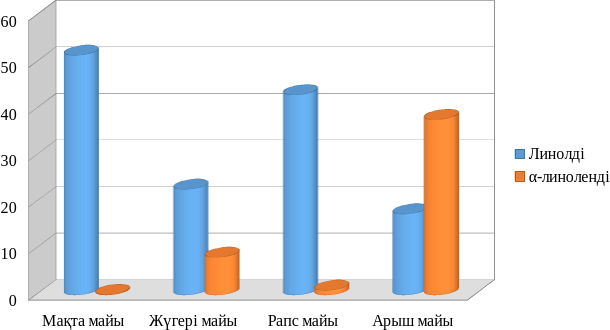
\includegraphics[width=0.8\textwidth]{assets/1107}
    \caption*{1-сурет - Майлардағы полиқанықпаған май қышқылдарының мөлшері}
\end{figure} (1)

Жүгері майының май қышқылдық құрамы (22 мас.\% линолен қышқылы және 8
мас.\% линолен қышқылы), ал арыш майы май қышқылдық құрамы (17,2 мас.\%
линолен қышқылы және 37,7 мас.\% линол қышқылы) бар және майлы майларды
пайдалана алады. Мақта майын байыту үшін қышқылдар өнеркәсібінде
қолданылуы мүмкін.

Көпкомпонентті май қоспаларының құрамын есептеу үшін линол және линолен
қышқылдарының қажетті қатынасын, сондай-ақ, майлардағы осы қышқылдардың
бастапқы құрамын ескеретін әдістеме қолданылды {[}10{]}. Есептеу (1)
және (2) формулалар бойынша жүзеге асырылады:

\begin{equation}
\frac{m_{a}\cdot c^{1}_{a}+m_{b}\cdot c^{1}_{b}}{m_{a}\cdot c^{2}_{a}+m_{b}\cdot c^{2}_{b}}=10;
\end{equation}
\begin{equation}
  m_{a}+m_{b}=1,
\end{equation}

Мұндағы,

\emph{m\textsubscript{a}}, \emph{m\textsubscript{b}} -- өсімдік майының
массасы, кг;

$c^{1}_{a}$, $c^{1}_{b}$ -- өсімдік майындағы линол қышқылының концентрациясы, мас. \%;

$c^{2}_{a}$, $c^{2}_{b}$ -- өсімдік майындағы линолен қышқылының концентрациясы,~мас. \%
{[}11,12{]}.

Жүргізілген есептеулер негізінде 3-кестеде ұсынылған май қоспалары
ұсынылды.

\begin{table}[H]
\caption*{3-кесте - Қоспалардағы өсімдік майларының мөлшері}
\centering
\begin{tabular}{|l|l|l|l|}
\hline
Объект номері & Полиқанықпаған май қышқылдары нақты қатынасы & Мақта майы & Арыш майы \\ \hline
Қоспа 3 & 10:1 & 0,88 & 0,12 \\ \hline
Қоспа 4 & 5:1 & 0,8 & 0,2 \\ \hline
Қоспа 5 & 3:1 & 0,65 & 0,35 \\ \hline
\end{tabular}%
\end{table}

\begin{multicols}{2}
Қоспалар зертханалық жағдайларда алдымен екі негізгі майды араластыру
(20°C температурада магниттік араластырғышты пайдаланып тұрақты
араластыру), содан кейін қоспалардың шағын компоненттерін енгізу арқылы
алынды.

Алынған өсімдік майларының қоспаларының үлгілері олардың
органолептикалық және физико-химиялық көрсеткіштерін анықтау үшін
зерттеулерден өтті (4-кесте).
\end{multicols}

\begin{table}[H]
\caption*{4-кесте - Аралас майлардың физика-химиялық көрсеткіштері}
\centering
\resizebox{\textwidth}{!}{%
\begin{tabular}{|p{0.15\textwidth}|p{0.15\textwidth}|p{0.15\textwidth}|p{0.15\textwidth}|p{0.15\textwidth}|p{0.15\textwidth}|}
\hline
Қоспа саны & Қышқылдық саны, мг КОН/г & Пероксид мәні, ½ O моль/кг & Ылғалдылық пен ұшқыш заттардың массалық үлесі, \% & Линол қышқылы құрамы, мас. \% & Линолен қышқылы құрамы, мас. \% \\ \hline
Қоспа 1 & 0,4 & 4,4 & 0,05 & 44,73 & 5,83 \\ \hline
Қоспа 2 & 0,5 & 4,7 & 0,06 & 42,68 & 7,27 \\ \hline
Қоспа 3 & 0,4 & 3,4 & 0,06 & 41,91 & 7,6 \\ \hline
НТҚА талаптары & 4 & 10 & 0,2 &  &  \\ \hline
\end{tabular}%
}
\end{table}

\begin{multicols}{2}
Барлық үлгілер үшін қышқыл және асқын тотығы сандары бойынша алынған
нәтижелер тазартылмаған тағамдық майлар қоспаларына қойылатын талаптарды
қанағаттандырды. Алайда, арыш майы бар үлгілерде қышқылдың да, асқын
тотығының да төмен мәндері бар екенін атап өткен жөн, бұл өндіруде,
құюда және сақтауда осы қоспалар үшін белгілі бір артықшылықтар береді.
Соған қарамастан, зерттеулердің нәтижелері өсімдік майларының барлық
ұсынылған қоспаларын өндіру мүмкіндігін дәлелдейді, өйткені олар
органолептикалық және физика-химиялық көрсеткіштері бойынша белгіленген
талаптарға толық сәйкес келеді.

Сонымен қатар, алынған өсімдік майларының қоспаларының құрамындағы ПҚМҚ
есептелген қатынасына сәйкестігі газ хроматографиясының көмегімен
бағаланды. 4 кестедегі мәліметтерден көрініп тұрғандай, линол және
линолен қышқылдарының арақатынасы күтілетін нәтижелерге толығымен сәйкес
келеді. Айта кету керек, соя майын қолданатын қоспалар әзірлеген
жағдайда, линолен қышқылына бай майларды енгізген жөн, бұл ПҚМҚ қажетті
арақатынасын қамтамасыз етуге мүмкіндік береді.

{\bfseries Қорытынды.} Сонымен қорытындылай келе, Қазақстан Республикасы
мен Ресей Федерациясының аумағында өсетін майлы дақылдардан алынатын
өсімдік майларының құрамы зерттелді. Триглицеридтердің май қышқылдарының
құрамын талдау өсімдік майларының ω-3 және ω-6 қышқылдарының қажетті
қатынасын қамтамасыз ете алмайтынын көрсетті, бұл өсімдік майларының
қоспаларын жасауды қажет етеді.

Қоспаларды алу үшін шикізат ретінде мақта және арыш майы сияқты майлар
ұсынылады. Сызықтық бағдарламалау әдісіне сүйене отырып, жұмыс
функционалды немесе профилактикалық өнім ретінде пайдалануға болатын екі
қоспаның композициясын ұсынады. Әзірленген қоспалардың композицияларына
әртүрлі пропорциядағы мақта мен арыш майы кіреді. Өсімдік майларының
қоспалары органолептикалық және физика-химиялық көрсеткіштері бойынша
белгіленген талаптарға толық сәйкес келеді. Өсімдік майларының ұсынылған
қоспаларының май қышқылдарының құрамын зерттеу адамға теңдестірілген
диетаны қамтамасыз ету үшін қажетті ω-3 және ω-6 ПҚМҚ қатынасына қол
жеткізілгенін көрсетті, бұл профилактикалық немесе емдік тамақтану үшін
қоспаларды күнделікті тұтынуға ұсынуға мүмкіндік береді.
\end{multicols}

\begin{center}
{\bfseries Әдебиеттер}
\end{center}

\begin{noparindent}
1. Пищевая химия / А.П. Нечаев, С.Е. Траубенберг, А.А. Кочеткова {[}и
др.{]}; под ред. А.П. Нечаева. -6-е изд., стер. - СПб.: ГИОРД, 2015.-
672 с. ISBN 978-5-98879-196-6

2. Коваленко Т.Д. Инновации в предприятиях пищевой промышленности:
разработка новых видов продуктов питания // Труды международного
симпозиума «Надежность и качество». -2011. - № 1. - С.184-185.

3. ОʼБрайен Р. Жиры и масла. Производство, состав и свойства, применение
/ Р.ОʼБрайен: пер. С анг.2-го изд. В.Д.Широкова, Д.А. Бабейкиной,
Н.С.Селидановой, Н.В.Магды - СПб.: Профессия, 2007. -752 с. ISBN
978-5-93913-123-0

4. Myhrstad M. C. W., Retterstol K., Telle-Hansen V. H. Effect of marine
n-3 fatty acids on circulating

inflammatory markers in healthy subjects
and subjects with cardiovascular risk factors// Inflamm Res. -2011.
-Vol. 60(4). -P. 309-319. DOI 10.1007/s00011-010-0302-5.

5. Fetterman J. W., Zdanowicz M. M. Therapeutic potential of n-3
polyunsaturated fatty acids in disease// Am J Health Syst Pharm. -2009.
-Vol. 66(13). -P. 1169-1179. DOI 10.2146/ajhp080411

6. Об утверждении Санитарных норм и правил «Требования к питанию
населения: нормы физиологических потребностей в энергии и пищевых
веществах для различных групп населения Республики Беларусь»:
постановление М-ва здравоохранения РБ, 20.11.2012, № 180 // Нац. реестр
правовых актов Респ. Беларусь. -2012. -№ 8/25580.

7. Нормы физиологических потребностей в энергии и пищевых веществах для
различных групп населения Российской Федерации. Методические
рекомендации. - М.: Федеральный центр гигиены и эпидемиологии
Роспотребнадзора. -2009. 38 с.

8. Табакаева О.В., Каланеик Т.К., Обогащенные растительные масла с
оптимизированным жирнокислотным составом // Масложировая промышленность.
-2007.-№2.-С.34-35

9. Жировые продукты для здорового питания. Современный взгляд / Л.Г.
Ипатова {[}и др.{]}. -М.: ДеЛи принт,2009. - 396 с.

10. Степычева Н.В., Фудько А.А. Купажированные растительные масла с
оптимизированным

жирно-кислотным составом // Химия растительного сырья.
-2011.-№ 2.- С. 27-33.

11. Владыкина Д.С., Ламоткин С.А., Колногоров К.П., Ильина Г.Н.,
Башарова А.О. Разработка купажей растительных масел со сбалансированным
жирнокислотным составом // Труды БГТУ. -2015. - № 4. -С. 240-246. ISSN
1683-0377.

12. Lauretani, F., Bandinelli, S., Bartali, B., Cherubini, A., Iorio, A.
D., Blè, A., Giacomini, V., Corsi, A. M., Guralnik, J.M., \& Ferrucci,
L. Omega-6 and omega-3 fatty acids predict accelerated decline of
peripheral nerve function in older persons. European journal of
neurology. -2007. --Vol. 14(7). -P:. 801-808. DOI
10.1111/j.1468-1331.2007.01860.x
\end{noparindent}

\begin{center}
{\bfseries References}
\end{center}

\begin{noparindent}
1. Pishchevaya khimiya / A.P. Nechaev, S.E. Traubenberg, A.A. Kochetkova
{[}i dr.{]}; pod red. A.P. Nechaeva. -- 6-e izd., ster. - SPb.: GIORD,
2015.- 672 s. ISBN 978-5-98879-196-6 {[}in Russian{]}

2. Kovalenko, T.D. Innovatsii v predpriyatiyakh pishchevoi
promyshlennosti: razrabotka novykh vidov produktov pitaniya // Trudy
mezhdunarodnogo simpoziuma «Nadezhnost\textquotesingle{} i kachestvo».
-2011. -- № 1. -- S.184-185. {[}in Russian{]}

3. OʼBraien R. Zhiry i masla. Proizvodstvo, sostav i svoistva,
primenenie / R.OʼBraien: per. S ang.2-go izd. V.D.Shirokova, D.A.
Babeikinoi, N.S.Selidanovoi, N.V.Magdy - SPb.: Professiya, 2007. -752 s.
ISBN 978-5-93913-123-0 {[}in Russian{]}

4. Myhrstad M. C. W., Retterstol K., Telle-Hansen V. H. Effect of marine
n-3 fatty acids on circulating

inflammatory markers in healthy subjects
and subjects with cardiovascular risk factors// Inflamm Res. -2011.
-Vol. 60(4). P. 309-319. DOI 10.1007/s00011-010-0302-5.

5. Fetterman J. W., Zdanowicz M. M. Therapeutic potential of n-3
polyunsaturated fatty acids in disease// Am J Health Syst Pharm. -2009.
-Vol. 66(13). -P. 1169-1179. DOI 10.2146/ajhp080411

6. Ob utverzhdenii Sanitarnykh norm i pravil «Trebovaniya k pitaniyu
naseleniya: normy fiziologicheskikh

potrebnostei v energii i pishchevykh
veshchestvakh dlya razlichnykh grupp naseleniya Respubliki
Belarus\textquotesingle»: postanovlenie M-va zdravookhraneniya RB,
20.11.2012, № 180 // Nats. reestr pravovykh aktov Resp.
Belarus\textquotesingle. -2012. -№ 8/25580. {[}in Russian{]}

7. Normy fiziologicheskikh potrebnostei v energii i pishchevykh
veshchestvakh dlya razlichnykh grupp naseleniya Rossiiskoi Federatsii.
Metodicheskie rekomendatsii. - M.: Federal\textquotesingle nyi tsentr
gigieny i epidemiologii

Rospotrebnadzora. -2009. 38 s. {[}in Russian{]}

8. Tabakaeva O.V., Kalaneik T.K., Obogashchennye
rastitel\textquotesingle nye masla s optimizirovannym zhirnokislotnym


sostavom // Maslozhirovaya promyshlennost\textquotesingle.
-2007.-№2.-S.34-35 {[}in Russian{]}

9. Zhirovye produkty dlya zdorovogo pitaniya. Sovremennyi vzglyad / L.
G. Ipatova {[}i dr.{]}. -M.: DeLi print,2009. - 396 s. {[}in Russian{]}

10. Stepycheva N.V., Fud\textquotesingle ko A.A. Kupazhirovannye
rastitel\textquotesingle nye masla s optimizirovannym zhirno-kislotnym
sostavom // Khimiya rastitel\textquotesingle nogo
syr\textquotesingle ya. -2011. -№2. -S. 27-33. {[}in Russian{]}

11. Vladykina D.S., Lamotkin S.A., Kolnogorov K.P.,
Il\textquotesingle ina G.N., Basharova A.O. Razrabotka kupazhei
rastitel\textquotesingle nykh masel so sbalansirovannym zhirnokislotnym
sostavom // Trudy BGTU. -2015. - № 4. -S. 240-246. ISSN 1683-0377. {[}in
Russian{]}

12. Lauretani, F., Bandinelli, S., Bartali, B., Cherubini, A., Iorio, A.
D., Blè, A., Giacomini, V., Corsi, A. M., Guralnik, J.M., \& Ferrucci,
L. Omega-6 and omega-3 fatty acids predict accelerated decline of
peripheral nerve function in older persons. European journal of
neurology. -2007. --Vol. 14(7). -P:. 801-808. DOI
10.1111/j.1468-1331.2007.01860.x
\end{noparindent}

\emph{{\bfseries Авторлар туралы мәліметтер}}

\begin{noparindent}
Отуншиева А.Е. - Әл-Фараби атындағы Қазақ Ұлттық университетінің
«Жылуфизика және техникалық физика» кафедрасы «Стандарттау және
сертификаттау» білім беру бағдарламасының докторанты, Алматы, Қазақстан,
e-mail: 03.08.1990.43@mail.ru;

Ламоткин С.А. - Беларусь мемлекеттік технологиялық университет,
«Физика-химиялық әдістер және сапаны қамтамасыз ету» кафедрасының
меңгерушісі, х.ғ.к., доценті,~ Минск, Беларуссия, e‑mail:
jossby@rambler.ru ;

Болегенова С.А. - Әл-Фараби атындағы Қазақ Ұлттық Университеті,
«Жылуфизика және техникалық физика» кафедрасының меңгерушісі,
ф.-м.ғ.д.,профессоры, Алматы, Қазақстан, e‑mail:
saltanat.bolegenova@kaznu.kz;

Ветохин С.С. {\bfseries -} Беларусь мемлекеттік технологиялық университеті,
«Физика-химиялық әдістер және сапаны қамтамасыз ету» кафедрасы,
ф.-м.ғ.к., профессоры, Минск, Беларуссия, e‑mail: serega49@mail.ru;

Ешанкулов А.А. {\bfseries -} М.Ауезов атындағы Оңтүстік Қазақстан Зерттеу
Университеті, «Механика және мұнайгаз ісі» факульетінің декан
орынбасары, «Стандарттау және сертификаттау» кафедрасының т.ғ.к.,
доценті, Шымкент, Қазақстан, e‑mail: amirkhan-74@mail.ru.
\end{noparindent}

\emph{{\bfseries Сведения об авторах}}

\begin{noparindent}
Otunshiyeva A.E.. - doctoral student of the educational programme
«Standardisation and Certification», department of «Thermal physics and
technical physics», Kazakh National University named after Al-Farabi,
Almaty, Kazakhstan, e-mail: 03.08.1990.43@mail.ru;

Lamotkin S.A. - Head of the Department «Physico-chemical methods and
quality assurance» of the Belarusian State Technological University,
Candidate of Chemical Sciences, Associate Professor, Minsk, Belarus,
e-mail: jossby@rambler.ru;

Bolegenova S.A. - Head of the Department of `Thermophysics and Technical
Physics', Kazakh National University named after Al-Farabi, Dr. Ph.
Almaty, Kazakhstan, e-mail: saltanat.bolegenova@kaznu.kz;

Vetokhin S.S. - Belarusian State Technological University, Department of
«Physico-chemical methods and quality assurance», Candidate of Physical
and Chemical Sciences, Professor, Minsk, Belarus, e-mail:
serega49@mail.ru;

Esankulov A.A. - deputy dean of the faculty «Mechanics and oil and gas
business» of M. Auezov South Kazakhstan Research University, Candidate
of Science, associate professor of the department `Standardisation and
Certification', Shymkent, Kazakhstan, e-mail: amirkhan-74@mail.ru.
\end{noparindent}
